\begin{refsection}

\chapter{Pb--Pb and Th--Pb}\label{ch:Th-Pb-Pb}

The Pb--Pb and Th--Pb methods are extensions of the U--Pb method that
do not require measuring uranium. Although Chapter~\ref{ch:U-Pb} did
discuss \textsuperscript{207}Pb/\textsuperscript{206}Pb ages and the
U--Th--Pb concordia diagram and isochron, the applications of
\textsuperscript{207}Pb/\textsuperscript{206}Pb and
\textsuperscript{208}Pb/\textsuperscript{232}Th discussed in this
chapter are suffiently different to warrant separate discussion.  The
Pb--Pb method applies the full
\textsuperscript{204}Pb--\textsuperscript{206}Pb--\textsuperscript{207}Pb
composition of cogenetic minerals to construct isochrons. This method
plays a fundamental role in unravelling the early history of the solar
system, and has been used to date the formation of our planet. The
Th--Pb method behaves very much like the Rb--Sr, Sm--Nd and other
simple parent daughter chronometers, which will be discussed in more
detail in Chapter~\ref{ch:PD}.

\section{Pb--Pb}\label{sec:PbPb}

Pb--Pb data can be supplied in three data formats:
\begin{enumerate}
\item{`Normal':}
  $\frac{06}{04}$,  
  $\mbox{err}\!\left[\frac{06}{04}\right]$, 
  $\frac{07}{04}$,  
  $\mbox{err}\!\left[\frac{07}{04}\right]$,  
  $\mbox{r}\!\left[\frac{06}{04},\frac{07}{04}\right]$
\item{`Inverse':}
  $\frac{04}{06}$,  
  $\mbox{err}\!\left[\frac{04}{06}\right]$, 
  $\frac{07}{06}$,  
  $\mbox{err}\!\left[\frac{07}{06}\right]$,  
  $\left(\mbox{r}\!\left[\frac{04}{06},\frac{07}{06}\right]\right)$
\item{`Three ratios':}
  $\frac{06}{04}$, 
  $\mbox{err}\!\left[\frac{06}{04}\right]$, 
  $\frac{07}{04}$, 
  $\mbox{err}\!\left[\frac{07}{04}\right]$, 
  $\frac{07}{06}$, 
  $\mbox{err}\!\left[\frac{07}{06}\right]$
\end{enumerate}

\noindent where format~3 can be converted to format~1 using
Equation~\ref{eq:redundantratios}. Format~1 can be converted to
format~2 using the following expression:
\begin{equation}
  \begin{cases}
    x' = \frac{1}{x} \\
    y' = \frac{x}{y} \\
    \left(\frac{s[x']}{x'}\right)^2 = 
    \left(\frac{s[x]}{x}\right)^2 \\
    \left(\frac{s[y']}{y'}\right)^2 =
    \left(\frac{s[x]}{x}\right)^2 -
    2 \rho_{x,y}\left(\frac{s[x]}{x}\right)\left(\frac{s[y]}{y}\right) +
    \left(\frac{s[y]}{y}\right)^2 \\
    \rho_{x'y'} =
    \left(\frac{x'}{s[x']}\right)
    \left[
    \left(\frac{y}{s[y]}\right) -
    \rho_{xy}\left(\frac{x}{s[x]}\right)
    \right]
  \end{cases}
  \label{eq:format12transformation}
\end{equation}

\noindent where $x=[06/04]$ and $y=[07/04]$, $x'=[04/06]$ and
$y'=[04/07]$. This transformation is perfectly symmetric in the sense
that it can also be used to convert inverse isochron ratios to
conventional ones, so that $x'=[06/04]$ and $y'=[07/04]$, $x=[04/06]$
and $y=[04/07]$.

\section{(inverse) isochrons}\label{sec:inverseIsochrons}

The `normal' and `inverse' monikers for the first two Pb--Pb input
formats refers to their use for isochron regression:

\begin{center}
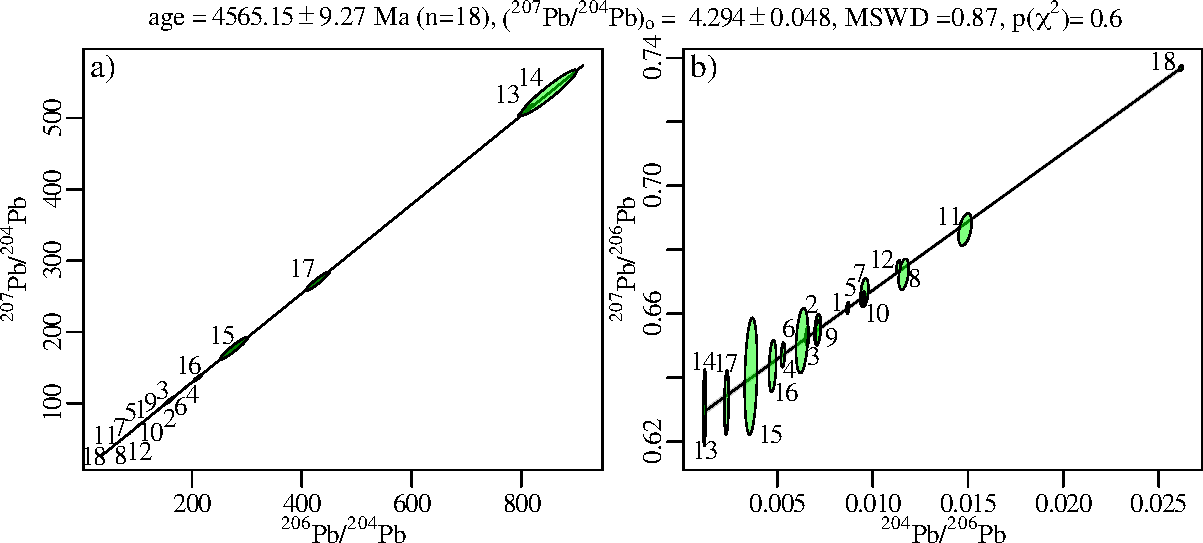
\includegraphics[width=.9\linewidth]{../figures/PbPb.pdf}\\ \captionof{figure}{a)
  conventional and b) inverse isochron plot for a Pb--Pb dataset of
  carbonaceous chondrules, which date the oldest meteorites in the
  solar system. The aliquots are numbered to facilitate the comparison
  of the two plots. The most radiogenic aliquots plot in the upper
  right corner of the conventional isochron, and in the lower left
  corner of the inverse isochron diagram. The conventional isochron
  places the least abundant isotope in the denominator,
  \textsuperscript{204}Pb, which caused strong error correlations for
  reasons that are explained in
  Section~\ref{sec:errorcorrelations}. These correlations are greatly
  reduced when the more abundant \textsuperscript{206}Pb is used as a
  common denominator.}
\end{center}

The Pb--Pb age is proportional to the slope of a conventional
isochron, and to the y-intercept of the inverse isochron. Conversely,
the \textsuperscript{207}Pb/\textsuperscript{204}Pb-ratio of the
common Pb is given by the y-intercept of the conventional isochron,
and by the slope of the inverse isochron. Provided that the analytical
uncertainties are reasonably small compared to the measured isotopic
ratios ($<5\%$, say), the age and common Pb composition are identical
for both approaches.

\section{The Stacey-Kramers growth curve}\label{sec:SKgrowth}

As previously discussed in Section~\ref{sec:common-Pb} and quantified
by Equations~\ref{eq:stacey-kramers-a}--\ref{eq:stacey-kramers-c}, the
mantle evolution model of \citet{stacey1975} describes the Pb
composition of the mantle through geologic time. This model can be
used for the common Pb correction of discordant samples, but can also
be used to compute `model ages' from Pb-rich mineral phases such as
galena. It is also useful to compare whole rock Pb--Pb isochron ages
with the mantle evolution model, in order to better understand the
source of the source material from which the rock was derived.  To
facilitate this type of investigation, \texttt{IsoplotR} allows the
\citet{stacey1975} growth curve to be plotted alongside the isochron
data, and estimates the intersection(s) between the isochron and the
growth curve.

\begin{center}
\noindent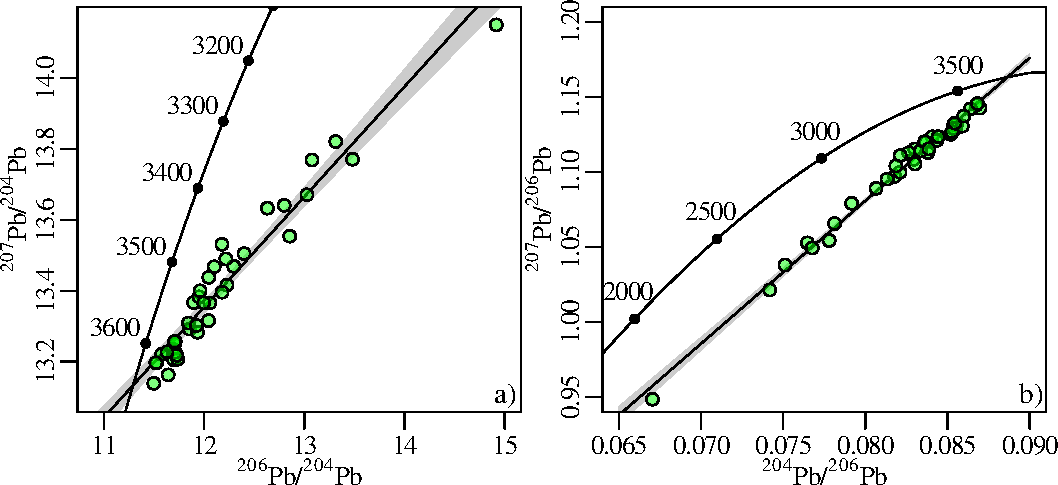
\includegraphics[width=.8\linewidth]{../figures/Kamber.pdf}
\captionof{figure}{a) conventional and b) inverse model-2 whole rock
  Pb--Pb isochron of the Am\^{i}tsoq gneiss
  \citep[Greenland,][]{kamber1998}, with the \citet{stacey1975} growth
  curve shown on the left.  The close agreement between the isochron
  age ($3550 \pm 130$~Ma) and the model age (3650~Ma) suggest that the
  magmatic precursor of the Am\^{i}tsoq orthogneiss was extracted from
  the mantle shortly before its formation.}
\label{fig:Kamber}
\end{center}

\section{Th--Pb}\label{sec:ThPb}

The Th--Pb method applies to minerals (such as allanite and monazite)
that are rich in Th and relatively poor in U. \texttt{IsoplotR}
accepts Th--Pb data in three formats that are similar to the Pb--Pb
data formats:

\begin{enumerate}
\item{`Normal':}
  $\frac{32}{04}$,  
  $\mbox{err}\!\left[\frac{32}{04}\right]$, 
  $\frac{08}{04}$,  
  $\mbox{err}\!\left[\frac{08}{04}\right]$,  
  $\mbox{r}\!\left[\frac{08}{04},\frac{08}{04}\right]$
\item{`Inverse':}
  $\frac{32}{08}$,  
  $\mbox{err}\!\left[\frac{32}{08}\right]$, 
  $\frac{04}{08}$,  
  $\mbox{err}\!\left[\frac{04}{08}\right]$, 
  $\left(\mbox{r}\!\left[\frac{32}{08},\frac{04}{08}\right]\right)$
\item{`Three ratios':}
  $\frac{32}{08}$,  
  $\mbox{err}\!\left[\frac{32}{08}\right]$, 
  $\frac{04}{08}$,  
  $\mbox{err}\!\left[\frac{04}{08}\right]$,  
  $\frac{32}{08}$,  
  $\mbox{err}\!\left[\frac{32}{08}\right]$
  $\frac{32}{04}$,  
  $\mbox{err}\!\left[\frac{32}{04}\right]$, 
\end{enumerate}

\noindent where format~3 can be converted to format~1 using
Equation~\ref{eq:redundantratios}, and format~1 can be converted to
format~2 (and vice versa) using
Equation~\ref{eq:format12transformation}. As the names of the formats
suggest, Th--Pb data can be used to form conventional and inverse
isochrons, where the former place non-radiogenic
\textsuperscript{204}Pb in the denominator, and the latter radiogenic
\textsuperscript{208}Pb:\\

\noindent\begin{minipage}[t][][b]{.7\linewidth}
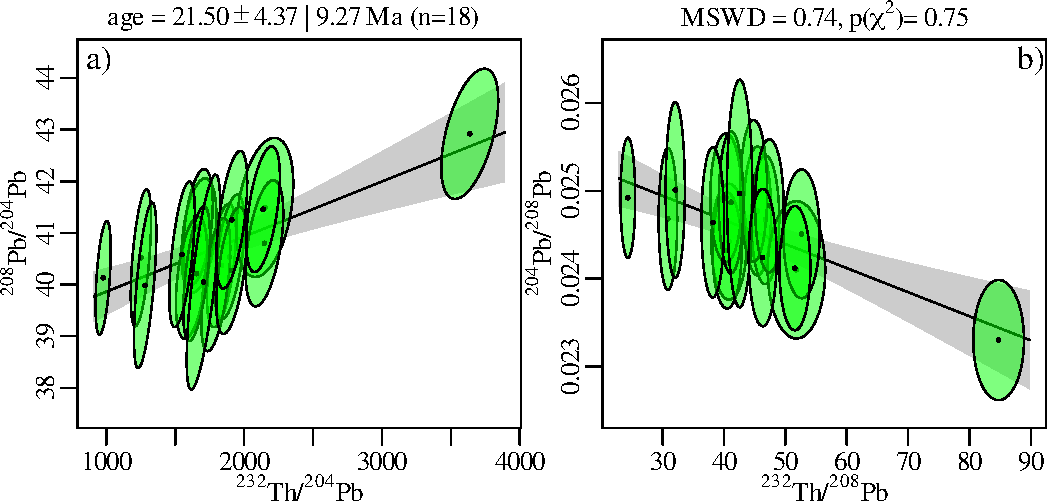
\includegraphics[width=\textwidth]{../figures/ThPb.pdf}
\end{minipage}
\begin{minipage}[t][][t]{.3\linewidth}
  \captionof{figure}{a) conventional and b) inverse model-1 isochron
    for the allanite Th--Pb data of \citet{janots2014}. The age is
    proportional to the slope of the conventional isochron, and to the
    x-intercept of the inverse isochron. The common-Pb composition is
    given by the y-intercept.}
  \label{fig:agediscordance}
\end{minipage}

\section{Single grain ages}\label{it:ThPbPbradial}

The Th--Pb method is usually applied to multiple aliquots from the
same sample, for which the isochron method can retrieve both the age
and the non-radiogenic Pb components. However it can also be useful to
inspect the ages of each individual aliquot, using radial plots, KDEs
and CADs. There are two ways to do this:

\begin{enumerate}
  \item Treat the aliquots together by projecting the isotopic ratio
    data onto the x-axis of the inverse isochron plot.
    \begin{equation}
      \left[\frac{D}{P}\right]_i^\ast = \frac{b}{b x_i - y_i}
      \label{eq:DP*inverse}
    \end{equation}
    
    \noindent where $[D/P]_i^\ast$ is the radiogenic
    daughter--to--parent ratio of the $i$\textsuperscript{th} aliquot,
    $x_i$ and $y_i$ are the independent and dependent variable of the
    inverse isochron diagram, and $b$ is its slope.

  \item Apply a nominal correction to each aliquot independently, by
    two point isochron regression. For example, in conventional
    isochron space:
    \begin{equation}
      \left[\frac{D}{P}\right]_i^\ast = \frac{y_i - y_\circ}{x_i}
      \label{eq:DP*conventional}
    \end{equation}

    \noindent where $y_\circ$ is the isotopic ratio of the inherited
    daughter component.
\end{enumerate}

\noindent\begin{minipage}[t][][b]{.65\linewidth}
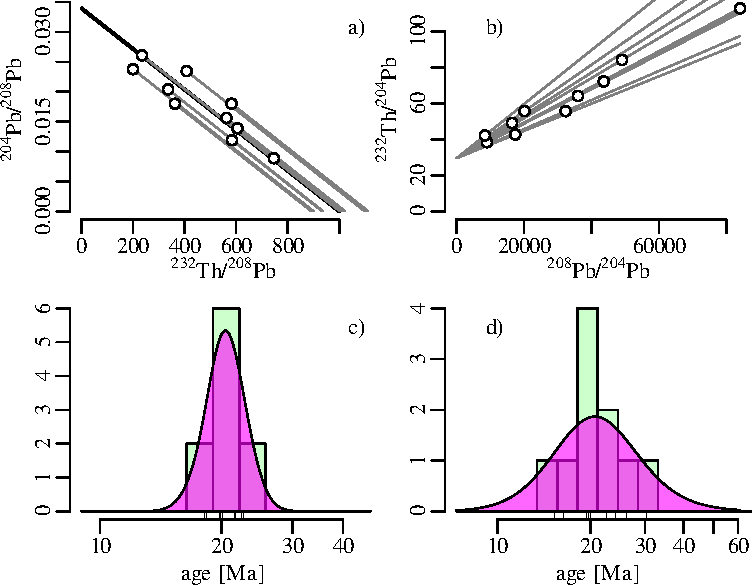
\includegraphics[width=\textwidth]{../figures/ThPbSingleGrain.pdf}
\end{minipage}
\begin{minipage}[t][][t]{.35\linewidth}
  \captionof{figure}{Single grain analysis of Th--Pb data by a)
    projecting each aliquot onto the x-axis of an inverse isochron,
    and b) individually correcting each aliquot by calculating the
    slope of a line that connects it to the common Pb composition on a
    conventional isochron diagram. The KDEs of the corresponding dates
    are shown in c) and d). The isochron-based approach yields less
    dispersed results.}
  \label{fig:ThPbSingleGrain}
\end{minipage}

\printbibliography[heading=subbibliography]

\end{refsection}
